\section{NDN-based Solution}
We propose an NDN-based solution to utilize intermediate results by caching them in NDN routers.  
Compared with IP-based Nectar, NDN-based solution integrates operations and input data into a name that can be used in matching cached data and routing the corresponding request to a producer of output data.
We first describe the system architecture in this section, and discuss further refinement in next section.

\subsection{Decompose Computation}
We observe that definition of intermediate results is the key to utlize intermediate results.
With this observation, we do not impose a language limitation in decomposing a program.
Instead, we allow users to define their own operations for decomposition, and use these operations.  
For example, given a computation program {\it P} shown in Figure \ref{fig:seq-eg}, it can be divided into three steps {\it A}, {\it B}, {\it C} based on its own logic.  
Each step can be defined as an operation in our design.  
Such a mechanism can provide users more flexibilities: 
1) a program written in other languages can still be decomposed;
2) users have full control over the decomposition instead of being limited by a low-level decomposer.  
We should also point out that although the steps in Figure \ref{fig:seq-eg} are sequential, a program does not have to be decomposed sequentially, as shown in Figure \ref{fig:non-seq-eg}.

\begin{figure}
\begin{center}
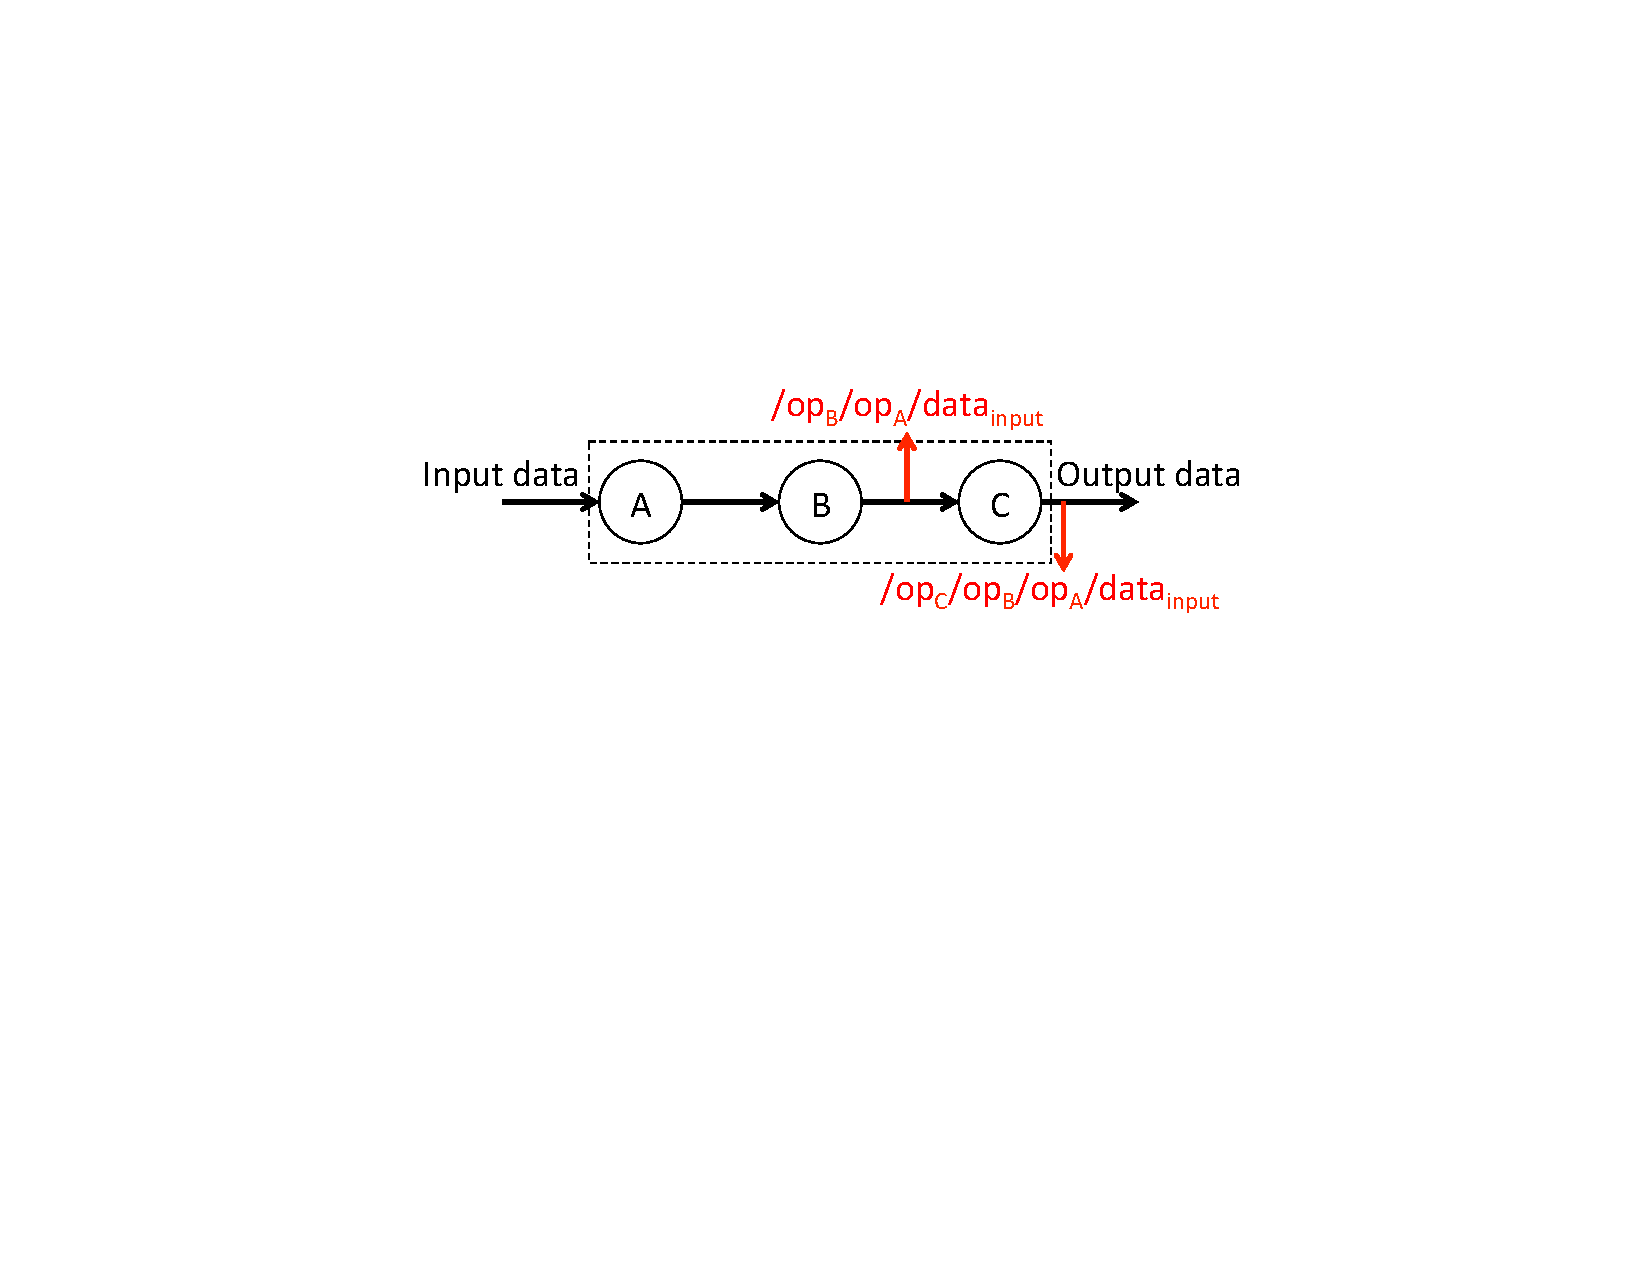
\includegraphics[width=0.5\textwidth]{fig-p-r/seq-eg.pdf}
\end{center}
\caption{A program is decomposed into three sequential operations.}
\label{fig:seq-eg}
\end{figure}

\begin{figure}
\begin{center}
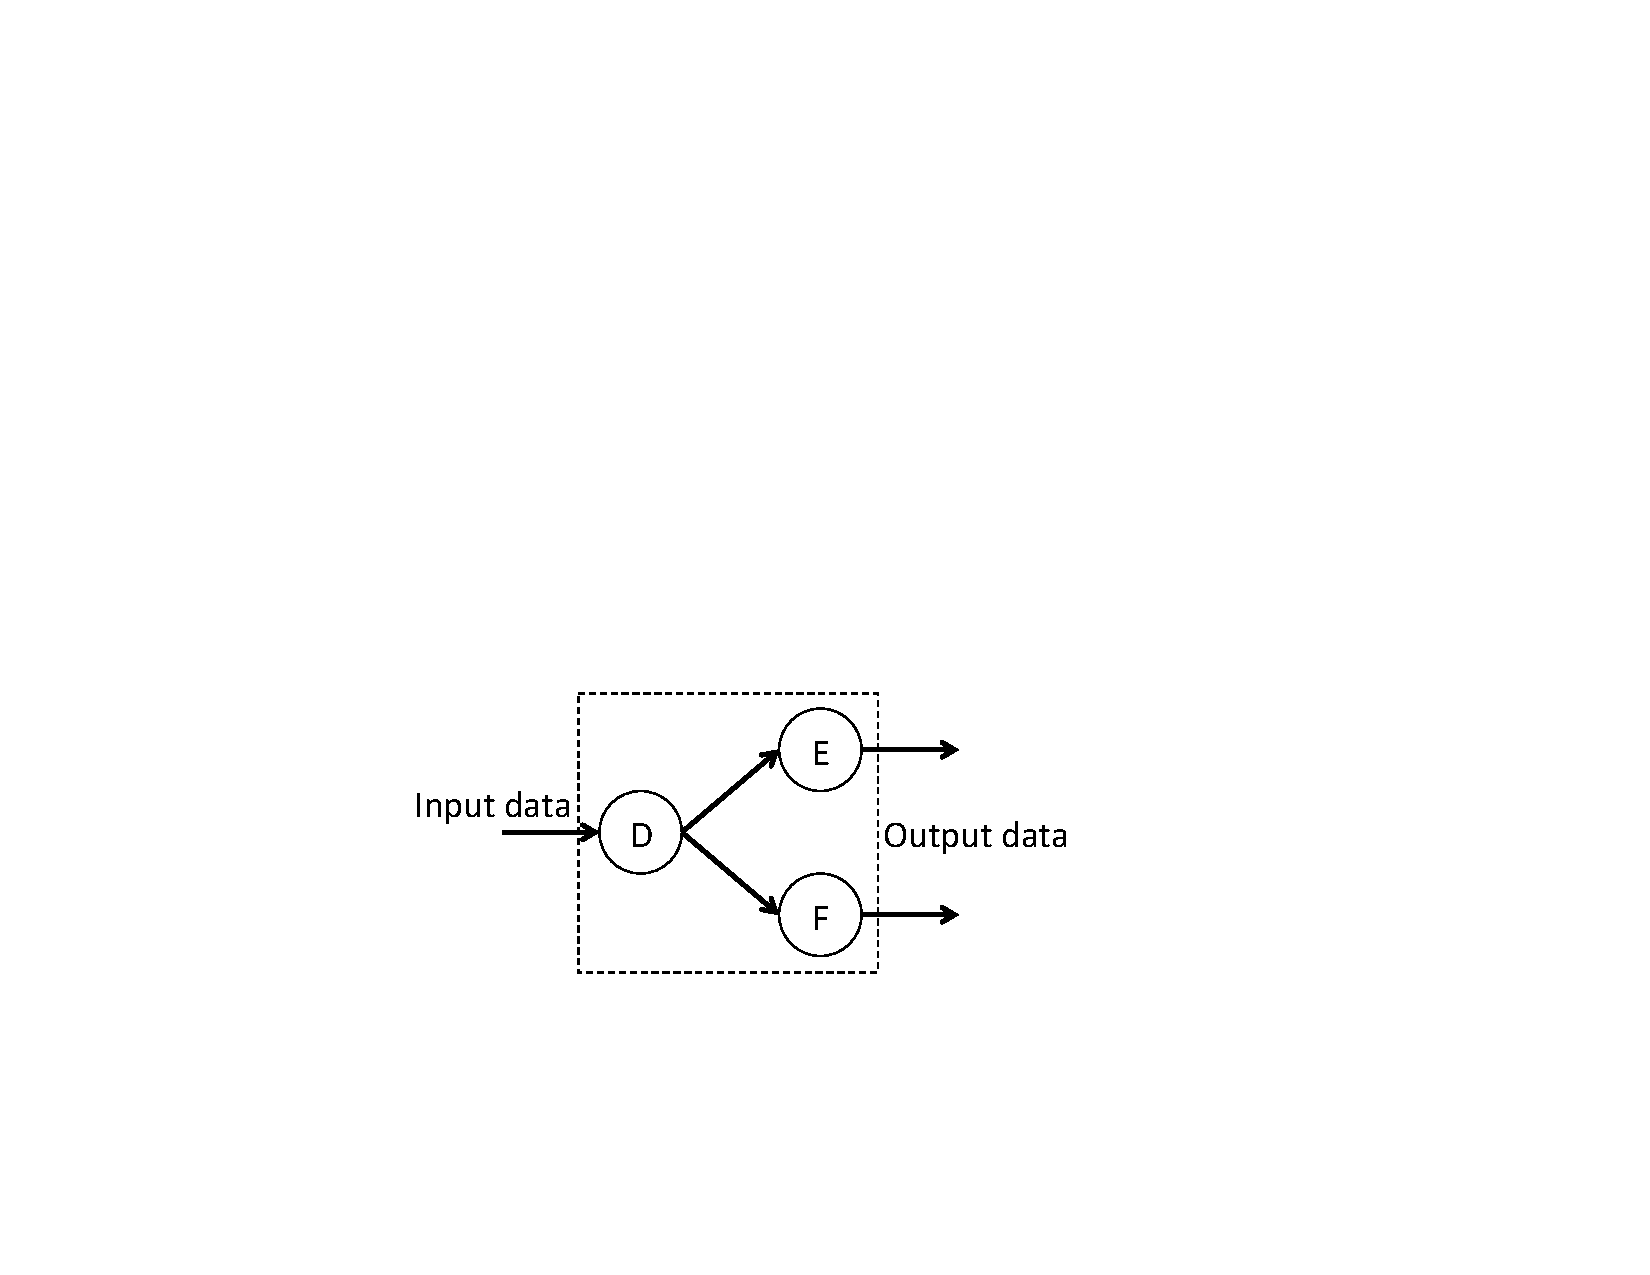
\includegraphics[width=0.4\textwidth]{fig-p-r/non-seq-eg.pdf}
\end{center}
\caption{A program is decomposed into three operations which is not sequential.}
\label{fig:non-seq-eg}
\end{figure}

\subsection{Identify Intermediate Results}
Although steps do not have to be sequential, intermediate results in our design are always identified as a sequential operations (e.g., $op_1$, $op_2$, ..., $op_N$) on a set of input data.  
The intermediate results can be named as following:
\begin{center}
/$op_N$/.../$op_2$/$op_1$/$<$InputDataName$>$
\end{center}
For example, in the example shown in Figure \ref{fig:seq-eg}, the intermediate result after operation {\it B} can be identified using name: /$op_B$/$op_A$/$data_{input}$.  
This name can be interpreted as ``it is the output result of performing operation {\it A} on input data $data_{input}$, and performing operation {\it B} on the result of operation {\it A}''.  
We can also generalize such a naming mechanism by including final output results.  
If the whole computation program is decomposed in a sequential way as shown in Figure \ref{fig:seq-eg}, the final output result can be identified as /$op_C$/$op_B$/$op_A$/$data_{input}$.  
For an unsequential decomposition, the final output result can be idenitified by several names.  
For instance, in Figure \ref{fig:non-seq-eg}, the final results can be expressed as:
/$op_E$/$op_D$/$data_{input}$ and /$op_F$/$op_D$/$data_{input}$.

\subsection{Compute Without Cache}
\begin{figure}
\begin{center}
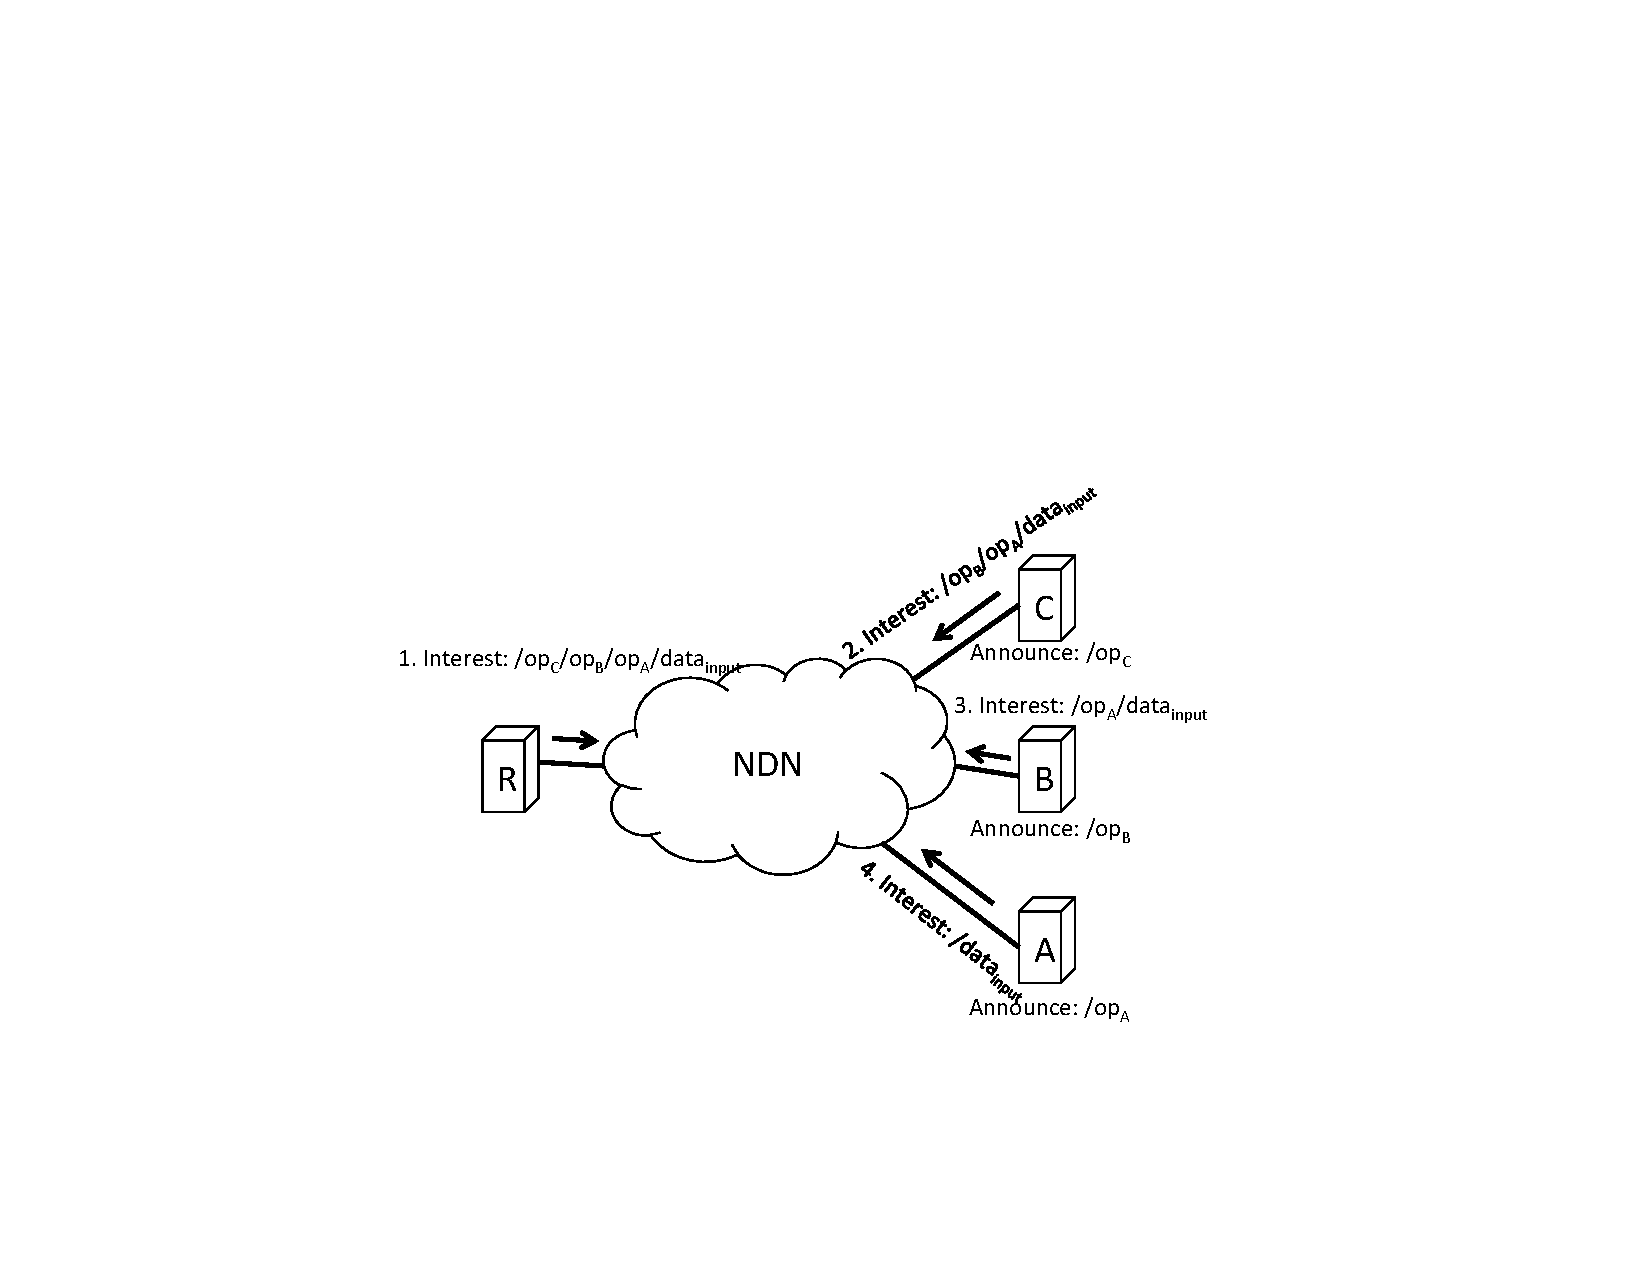
\includegraphics[width=0.5\textwidth]{fig-p-r/cpt-wo-cache.pdf}
\end{center}
\caption{An example of distributed computing in NDN without using cache.}
\label{fig:cpt-wo-cache}
\end{figure}
We first describe how NDN-based network supports distributed computing, then describe how to enhance the distributed computing by using cached intermediate results in next section.  
The computation program shown in Figure~\ref{fig:seq-eg} is used as an example to illustrate the whole procedure.
The first step is to deploy the decomposed operations (e.g., {\it A}, {\it B}, {\it C}) on servers.  
As shown in Figure~\ref{fig:cpt-wo-cache}, each operation is deployed on one server. However, multiple operations can share one server, and one operation can be deployed on multiple servers as we will discuss in Section~\ref{sec:robust}.  
A server with a operation deployed should announce a name prefix indicating its capability of performing the operation.  
For example, server $S_B$ in Figure \ref{fig:cpt-wo-cache} announces a prefix ``/$op_B$'', the server should be able to perform operation {\it B}.  
Therefore, all {\sc interest} messages with names sharing the prefix ``/$op_B$'' (e.g., ``/$op_B$/$op_A$/$data_{input1}$'' and ``/$op_B$/$data_{input2}$'') will be
forwarded to the server $S_B$.  When $S_B$ receives an {\sc interest} meassage with ``/$op_B$'' as the name prefix, it treats the suffix following ``/$op_B$'' (e.g., ``/$op_A$/$data_{input1}$'' and ``/$data_{input2}$'' in previous examples) as the name of the input data for it to perform operation {\it B}.  
If $S_B$ does not have the input data for operation {\it B}, it will send another {\sc interest} message using the suffix as the name.  
If the suffix involves another operation, for example, operation {\it A} in suffix ``/$op_A$/$data_{input1}$'', the {\sc interest} message will be forwarded to server $S_A$, which annonuces prefix ``/$op_A$'' (i.e., the server with operation $A$ deployed), and $S_A$ can use an {\sc interest} with the name ``/$data_{input1}$'' to fetch the initial input data.  
In this way, the original {\sc interest} message (e.g., /$op_B$/$op_A$/$data_{input1}$) can recursively trigger $S_A$ to perform operation {\it A} and $S_B$ to perform operation {\it B} once upon $S_A$ has finished its computation, and the {\sc data} message which eventually satisfies the original {\sc interest} message should contains the desired final output result.

\subsection{Utilize Cached Results} \label{sec:utilize_cache}
As {\sc data} packets can be cached in NDN network, or more specifically speaking in NDN routers, incoming {\sc interest} packets can be satisfied by cached {\sc data} packets, instead of asking data producers (e.g., computation servers deployed with operations in this paper) to generate data again.  
Since cached data can be matched with the names carried in {\sc interest} packets, when a NDN router receives an {\sc interest} packet, it first lookup its local cache.  
If there is a cache hit, then the cached data can be used to satisfy the {\sc interest}.  
Otherwise, it forwards the {\sc interest} packet to a neighbour NDN router which via routing protocol claims that it knows how to reach the corresponding data producer (the computation server announcing a prefix of the name in the {\sc interest} packet).  
As {\sc data} packet always flows back along the way {\sc interest} packet goes, it is still possible for the {\sc interest} packet to find a cache hit in the neighbour router.

However, without a careful design, the cache may not perform very effectively. 
For example, a data requester (a server that is about to perform an operation in this paper) may request an intermediate result which shares the the same operation sequence with some other intermediate results computed previously, but their input data sets are different. 
In order to maximize the caching efficiency, we have to solve three problems:
\begin{enumerate}
\item How to match cached data without using the exactly same name?
\item How to represent requested input data set in a hierarchical name?
\item How to find out all available data that has already been cached?
\end{enumerate}

The first problem is the most difficult one.  
The longest-prefix match restricts the name to be hierarchical.  
Data sets, however, may differ a lot, no matter in terms of dimensions or granularities.  
It is not feasible to use a hierarchical name as a generalized way to represent various data sets.  
It is more reasonable for applications to define their own naming conventions to optimize performance.
Therefore, in our design we only use the exactly same name to match cached data.

With this assumption, we consider the next two problems.  
There are two different strategies to represent data sets.  
The first strategy is to divide data set with a unified granularity and represent each unit using a name.  
When a data requester needs output results of a specific operation sequence over an input data set.  
It divides the input data set into several units, and send {\sc interest} packets for output results over each data unit.  
However, it is difficult to define the granularity of a data unit.  
A too coarse granularity can reduce the caching efficiency, while a too fine granularity can leads to a significant amount of packets exchanging and a huge number of cache entries.
Even worse, the number of cache entries increases as intermediate results are accumulated.  
The second strategy is to put the range of data set into the name, therefore a data set is represented by one name.  
Although the scale of packet exchanging and cache entries can be significantly reduced, it makes the third problem more difficult.  
We propose a solution that combines the good features of the two strategies and avoid their defects by introducing an extra metadata fetching.

In our solution, before the data requester sends out {\sc interest} for intermediate results, it first sends an {\sc interest} with name 
\begin{center}
/\textless{\it operation\_sequence}\textgreater/{\it DataNameSet}/\textless{\it input\_range}\textgreater
\end{center}
to collect names of existing intermediate results which is related to the input data set.  
The returned {\sc data} is called ``metadata'' which consists of a name set of intermediate results. 
Each name in the name set has its own input data range.
The data ranges of all names in the name set construct a partition of the original input data range.
Some names in the set refer to intermediate results that have already been computed, while the others have not been computed yet.
Although which existing intermediate results should be used to make a partition is determined by computation server,
such a partition should indicate the most cost-saving plan for the operation sequence indicated in the name.  
The TTL of this metadata {\sc data} packet is set to 0, so that it will never be cached in a router.  
As a result, all the {\sc interest} packets for metadata will be forwarded to the server which is responsible for the first component in the {\it operation\_sequence} of the name (i.e., the last operation in the sequence of operations).  
For example, a metadata {\sc interest} ``/$op_C$/$op_B$/$op_A$/{\it DataNameSet}/1-100'' will be eventually forwarded to server $S_C$ which is responsible for operation $C$.  
And it will be divided by the computation server $S_C$ according to its previous computation results and its computation policy into three pieces: ``/$op_C$/$op_B$/$op_A$/1-30'', ``/$op_C$/$op_B$/$op_A$/31-40'' and ``/$op_C$/$op_B$/$op_A$/41-100''. 
Since server $S_C$ handles all computation of operation $C$, it always knows which intermediate data has been computed if $S_C$ keeps a record for it.  
Therefore, given a specific input data range, server $S_C$ can determine a set of intermediate results that is most cost-saving, and return their names via the metadata {\sc data} packet.

Once the data requester gets the name list from the metadata, it simply uses these names to fetch intermediate results.
For intermediate results that have been computed before and exist in the cache of NDN routers, the {\sc interest} messages with their names can be automatically satisfied by the cached content.
For intermediate results that have not been computed yet, or expired in the cache of NDN routers, the {\sc interest} messages will experience a serial of cache misses, but will eventually arrive the holder of the intermediate results (e.g., computation servers, or Repo), or the generator of the intermediate results (e.g., computation servers). 
The generator can repeat previous procedure to query the most cost-saving plan for its own input intermediate results.

There are three more benefits of asking computation servers for name list.  
First, intermediate results do not have to be in the same granularity.  
Second, computation servers can keep statistics for intermediate results, thus telling which one should be cached for a long time, and which one is no longer needed. 
This information is very useful for garbage collection as we will discuss in Section \ref{sec:gg}.
Third, computation server can merge intermediate results as necessary. We will discuss intermediate results merging in Section \ref{sec:merge}.
